\documentclass[a4paper,10pt]{article} 
\usepackage[margin=1in]{geometry}

\usepackage{amsmath}
\usepackage{amsthm}
\usepackage{amssymb}
\usepackage{enumitem}
\usepackage{mathrsfs}
\usepackage{amssymb}
\usepackage{hyperref}
\usepackage{graphicx}
\usepackage{minted} % código no latex
\usepackage[utf8]{inputenc} % pseudocódigo no latex
\usepackage[linesnumbered,ruled,vlined]{algorithm2e} % pseudocódigo no latex

\title{Relatório sobre a implementação do bootstraping amortizado}
\author{
    Aluno: Gustavo Esteche Araujo\\
    Orientador: Prof. Hilder Vitor Lima Pereira
}
\date{}

\usepackage[portuguese]{babel}
% Definitions in Portuguese
\numberwithin{equation}{section} % Opcional, se quiser equações numeradas por seção

% comandos de atalhos
\newcommand{\mcR}{\mathcal{R}}
\newcommand{\RLWE}{\text{RLWE}}

% Define o estilo e a numeração por seção
\newtheorem{theorem}{Teorema}[section]
\newtheorem{lemma}[theorem]{Lema}
\newtheorem{proposition}[theorem]{Proposição}
\newtheorem{corollary}[theorem]{Corolário}

\theoremstyle{definition}
\newtheorem{definition}[theorem]{Definição}

\begin{document} 

\maketitle

\section{Introdução}
\textbf{Aviso}: Ao comparar com o relatório parcial, note que este relatório melhora partes presentes no anterior e adiciona os progressos feitos na pesquisa. 
Para ver apenas o que foi substancialmente melhorado ou adicionado, comece a leitura pela seção 4 sobre duais. O código foi suprimido em várias seções por razões 
de comprimento, cheque o github para mais detalhes.

Neste relatório está escrito o que foi produzido em relação a pesquisa sobre a implementação do 
bootstraping amortizado descrito em \cite{lw23I} e \cite{lw23II}. A parte inicial da pesquisa se 
resumiu a um estudo de nivelamento sobre álgebra abstrata, para melhor compreender os objetos 
matemáticos relacionados à pesquisa. A pesquisa prosseguiu com a implementação das operações essenciais para 
viabilizar o bootstrapping proposto, de modo que os algoritmos descritos nos artigos pudessem, por fim, ser integralmente 
implementados e, assim, ter sua viabilidade de utilização devidamente analisada. 
O relatório foi produzido 
compilando os resultados de cada seção individual. Para acessar o conteúdo escrito e acessar também as implementações e testes,
segue o link para o github \url{https://github.com/gustavoesteche/ic-bootstraping}.

\subsection{Traço}
Seja $K \subseteq L $ um extensão de corpo finito e $Aut_K(L)$ o subconjunto de automorfismos
de $L$ que fixam elementos de $K$, ou seja, se $\sigma \in Aut_K(L)$ e $\alpha \in K$, logo $\sigma(\alpha) = \alpha$. Então o Traço de $L$ em $K$ de um elemento $a \in L$ é definido por 
\begin{equation}
    Tr_{L/K}(a) = \sum_{\sigma \in Aut_K(L)} \sigma(a)  
\end{equation} 
Então, computar o traço se resume a encontrar os automorfismos que fixam os elementos.

Sendo $p$ um primo e $n \in \mathbb{Z}^{+}$, considere o anel ciclotômico  
$R_{p^n} = \mathbb{Z}[x]/<\Phi_{p^n}(x)>$. Semelhante a seção anterior, este anel também pode ser escrito como $\mathbb{Z}(\zeta_{p^n})$, onde o isomorfismo é $x \mapsto \zeta_{p^n}$.

Inicialmente, foi encontrado como computar o traço de um elemento $a$ entre os anéis $R_{p^n}$ e $R_{p^{n-1}}$, denotado como $Tr_{R_{p^n}/R_{p^{n-1}}}$.
Observe que o problema foi definido sobre os corpos e não anéis, porém como o automorfismo respeita a estrutura do anel, portanto o traço permanece bem definido. Os automorfismos em anéis ciclotômicos são da forma $X \mapsto X^i$, então, para encontrar os automorfismos basta encontrar os expoentes que satisfazem a propriedade de fixação requerida. 
Vamos separar em dois casos:

\paragraph{Caso 1: $n=1$} 
    Esta discussão é trivial, porque teremos apenas $\varphi(p) = p-1$
    automorfismos, que serão definidos por todos os expoentes coprimos com $p$,
    ou seja $[1,p-1]$. Logo, os automorfismos são $\sigma_i(X) = X^i$.

\paragraph{Caso 2: $n>1$} 
Definimos um conjunto de $\varphi(p^n)/\varphi(p^{n-1}) = p$ automorfismos do anel $\mathbb{Z}[x]/\langle \Phi_{p^n}(x) \rangle$ sobre $\mathbb{Z}[x]/\langle \Phi_{p^{n-1}}(x) \rangle$, dados por:
\[
\sigma_k(x) = x^{k p^{n-1} + 1}, \quad 0 \leq k \leq p-1.
\]
Se $g(x) \in R_{p^{n-1}}$, ou seja, $g(x) = \sum_{i=0}^{\varphi(p^{n-1})} b_i \zeta_{p^{n-1}}^i$. Usando $\zeta_{p^{n-1}} = \zeta_{p^n}^p$, $\sigma_k(g(x))$ pode ser escrito como:
\[
\sigma_k(g(x)) = \sum_i b_i x^{pi(k p^{n-1} + 1)} = \sum_i b_i x^{p i k p^{n-1}} x^{pi}.
\]

Como $x^{p i k p^{n-1}} = (x^{p^n})^{ik} \equiv 1 \mod \Phi_{p^n}(x)$, segue que $\sigma_k(g(x)) = g(x)$. Portanto, os automorfismos $\sigma_k$ \emph{fixam} o subanel $R_{p^{n-1}}$.

Seja $f(x)$ um polinômio em $R_{p^n}$ escrito como 
$
f(x) = \sum_{i=0}^{\varphi(p^n)/p} x^{pi} \sum_{j=0}^{p-1} a_{ij} x^j.
$ podemos simplificar a atuação do traço de $R_{p^n}$ para $R_{p^{n-1}}$:

\[
\sum_{k=0}^{p-1} \sigma_k(f(x)) = p \sum_{i=0}^{\varphi(p^n)/p} x^{pi} a_{i0}.
\]
Esse traço pode ser aplicado recursivamente por uma torre:
$
R_{p^n} \longrightarrow R_{p^{n-1}} \longrightarrow \cdots \longrightarrow \mathbb{Z},
$
permitindo computar traços intermediários até o corpo base, ou até o corpo necessário, operação implementada em SageMath.

Ademais, foram obtidas expressões explícitas para os traços parciais $\mathrm{Tr}_{K/K_{12}}$ e $\mathrm{Tr}_{K/K_{13}}$, fundamentais para o \textit{framework} de \textit{batch bootstrapping} apresentado em \cite{lw23I}. Seja $K = K_1 \otimes K_2 \otimes K_3$ e $K' = \bigotimes_{l \neq q} K_l$, então, para $a = \bigotimes_l a_l \in K$, usando a equação [\ref{eq:ring_embeddings}] foi demonstrado que:

\begin{equation}
    \mathrm{Tr}_{K/K'} (a) = \left( \bigotimes_{l \neq q} a_l \right) \cdot \mathrm{Tr}_{K_q/\mathbb{Q}} (a_q)
\end{equation}

Essa fórmula permite computar o traço parcial removendo um dos fatores do produto tensorial de corpos, simplificando significativamente sua implementação algébrica, que foi usado para critério de confirmação da solução polinômial e pode ser utilizada no futuro para otimização da implementação proposta, foi implementada em SageMath.

Em vias de fato, os tensores são uma das representações do que 
na realidade é representado por um polinômio $f(x) \in K$. No desenvolvimento a seguir vamos tratar novamente do caso onde queremos eliminar um corpo do traço, ou seja,
fixar os elementos dos outros corpos. Tome os mesmos corpos definidos anteriormente. Como $K$ é dado por um produto tensorial, para $f(x) \in K$ temos:  
$$
f(x) = \sum_i^{\phi(m1)-1} a_i x^{im_2m_3} \times \sum_j^{\phi(m2)-1} b_j x^{jm_1m_3} \times \sum_k^{\phi(m3)-1} c_i x^{km_1m_2}
$$ 
onde cada termo estava originalmente em $K_1,K_2, K_3$ respectivamente. Assuma sem perda de generalidade que queremos fixar os elementos dos dois primeiros corpos.
logo, o automorfismo $a$ tem a forma: 
$$
 x^{a(im_2m_3 + jm_1m_3)} = x^{im_2m_3 + jm_1m_3}
$$
Então $a m_2 m_3 \equiv m_2 m_3 $ e $a m_1 m_3 \equiv m_1 m_3$, para isso $a = k \times m_1 m_2$. Porém, é importante que $a m_1 m_3 \not\equiv m_1 m_3$, portanto
temos que remover esses múltiplos apropriadamente. A solução pode ser vista no seguinte pseudocódigo:

\begin{algorithm}[H]
\caption{Cálculo dos automorfismos}
\KwIn{Inteiros $m$, $p$, $n$}
\KwOut{Lista de automorfismos}

$rest \gets \{\, i \in [0, p-1] \mid i \neq k \,\}$ \;
$aut \gets \emptyset$ \;

\For{$i \gets 0$ \KwTo $p^{n-1} - 1$}{
    \ForEach{$j \in rest$}{
        $a \gets (i \cdot p + j) \cdot m / p^n + 1$ \;
        adiciona $a$ a $aut$\;
    }
}
\Return $aut$
\end{algorithm}

Tais automorfismos são aplicados na definição de traço para seu cálculo na implementação. Esta função foi implementada em SageMath e C++.

\newpage

\section{Composição de Anéis}
\subsection{Objetivo}
A ideia principal é entender como representar elementos em um anel maior usando de elementos em anéis menores para computação mais rápida, e então implementar/testar algumas propriedades derivadas.   

\subsection{Ferramentas Matemáticas}

\subsubsection{Definições}
Para o nosso problema, considere um inteiro $m$, então será analisado como compor o anel quociente $R_{m} = \mathbb{Q}[X]/ <\Phi_{m}(X)>$ utilizando anéis quocientes menores. 
Observe que este anel quociente também é um corpo, já que $\mathbb{Q}$ é um corpo, e por definição toda raiz de $\Phi_m(x)$ está em $\mathbb{C}$, então
$\Phi_m(x)$ é um polinômio irredutível sobre $\mathbb{Q}$, logo $R_{m} = \mathbb{Q}[X]/ <\Phi_{m}(X)>$ é um corpo. Outra definição útil é: seja $K_m$ a extensão de corpo tal que $K_m  = \mathbb{Q}(\zeta_m)$. É trivial ver que  $R_m \cong K_m$, pelo isomorfismo $X \mapsto \zeta_m$, portanto o desafio
de decompor $R_m$ é essencialmente o mesmo que decompor $K_m$.

\subsubsection{Base de Potências}
A base de potências ou base canônica dos polinômios é a base trivial de polinômios, podendo assim ser usada para definir os elementos no anel quociente $R_{m} = \mathbb{Q}[X]/ <\Phi_{m}(X)>$. Para qualquer inteiro $m$, a base pode ser escrita como $B = \{1, x, x^2, ..., x^{\phi(m)-1}\}$ e, é claro, cada elemento da base é linearmente independente e o 
envoltório linear da base é igual a todos os possíveis elementos em $R_{m}$. Como $R_m \cong \mathbb{Q}(\zeta_m)$, a base de potências também pode ser vista como $\{1, \zeta_m, \zeta_m^2, ..., \zeta_m^{\phi(m)-1}\}$, 
devido ao isomorfismo mencionado anteriormente.

\subsubsection{Composição via produto tensorial e \textit{Powerful basis}}
Seja $m$ um inteiro com fatoração em primos $m = \prod_{l} m_l$ onde cada $m_l$ é uma potência de primo. Conforme descrito em \cite{lyubashevsky2013}
o corpo $K_m = \mathbb{Q}(\zeta_m)$ é isomorfo ao produto tensorial: 

\begin{equation}
    K_m \cong \bigotimes_l K_{m_l}
\end{equation}

De forma equivalente, em termos dos anéis polinomiais é possível vê-lo como

\begin{equation}
    K_m \cong \bigotimes_l \mathbb{Q}[X_l] / <\Phi_{m_l}(X_l)> 
\end{equation}

Adotando a interpretação polinomial de $K_m$ a partir da equação anterior, para fins de concretude, note que uma base natural sobre $\mathbb{Q}$ é o conjunto 
de multinômios $\prod_l X_l^{j_l}$ para cada escolha de $0 \le j_l < \phi(m_l)$, e como $\phi(m) = \prod_l \phi(m_l)$ esta escolha pode ser feita.
Este conjunto é chamado de \textit{"powerful" basis} de $K_m$.

A \textit{powerful basis} $\vec{p}$ de $K_m = \mathbb{Q}(\zeta_m)$ pode ser definida como o produto tensorial das bases de potências(ou \textit{powerful}) $\vec{p_l}$ de cada $K_{m_l}$. Note
que o conjunto de índices no tensor resultante do produto tensorial pode ser achatado, resultando em um tensor de \textit{rank} 1, conforme visto em \cite{lyubashevsky2013}.
Entretanto, o que realmente importa no cenário proposto é como efetivamente realizar o produto tensorial entre os elementos dos anéis $R_{m_l}$.

Agora, para uma descrição mais concreta de como realizar a composição, o produto tensorial externo atuará como uma multiplicação polinomial 
e o isomorfismo que mapeia cada $X_l$ em $X$ será: $X_l \mapsto X^{m/m_l}$. Este isomorfismo pode parecer um tanto não natural, mas ao observar a raiz
da unidade isso se torna mais natural, pois $\zeta_{m_l} = \zeta_m^{m/m_l}$. O mesmo procedimento pode ser feito para encontrar a mencionada
\textit{powerful basis} achatada. Por exemplo, para $m = 15$, $p_3 = \{1,x_{3}^1\}$ e $p_5 = \{1,x_{5}^1, x_{5}^2, x_{5}^3\}$,
depois de realizar os cálculos, a base resultante será $p = \{1, x^3, x^5, x^6, x^8, x^9, x^{11}, x^{14}\}$ mais uma vez confirmada pelo artigo \cite{lyubashevsky2013} após o isomorfismo $x \mapsto \zeta_m$. 

\subsubsection{Decomposição do Anel}
Na seção anterior descrevemos como efetuar a composição de elementos dos corpos $K_{m_l}$ em um elemento no corpo $K_m$.
Portanto, seria natural tentar realizar o caminho inverso, encontrando uma forma explícita de decompor um elemento em $K_m$ nos seus correspondentes em cada $K_{m_l}$. 
Mas acontece que não existe uma operação de produto tensorial "inversa" trivial. Isso pode ser visualizado pelo seguinte: sejam $A$ e $B$ duas matrizes e $\psi$ tal que $\psi = A \otimes B$. 
Usando notação da soma de índices:

\begin{equation}
    \psi_{ijkl} = A_{ki} B_{jl}
\end{equation}

Usando qualquer $\lambda$ não-nulo no corpo no qual as operações estão definidas, temos $\psi_{ijkl} = (\lambda A_{ki}) (\lambda^{-1}B_{jl})$, portanto não há unicidade da solução. Alguém poderia argumentar que ao operar no anel dos inteiros,
apenas $1_{R}$ teria um inverso, levando a apenas três representações. Mas ao invés disso, podemos propor um problema clássico de álgebra linear: Note que, como os valores em $\psi$ são arbitrários, temos $|\psi| = |A||B|$ elementos a serem representados,
e apenas $|A| + |B|$ elementos de variáveis, então podemos até chegar a um caso degenerado, onde não há uma decomposição válida a ser proposta. Felizmente, este problema não parece ter aplicação no desenvolvimento do batch bootstrapping proposto,
então por enquanto será ignorado.

\subsection{Propriedades}

A partir da composição por produto tensorial surgem algumas propriedades interessantes, como segue:

\subsubsection{Propriedades de produto misto}
Assuma que $K, L$ são extensões de corpo de $\mathbb{Q}$, e que $a \in K$, $b \in L$. Então o produto tensorial de corpos $K \otimes L$ é definido como o conjunto de todas as combinações $\mathbb{Q}$-lineares de tensores puros $a \otimes b$, onde o produto tensorial
é bilinear em relação aos racionais, essas operações concebidas no produto tensorial de corpos devem satisfazer a propriedade de produto misto, i.e.,

\begin{equation}
    \label{eq:four_operations}
    \begin{split}
        (a_1 \otimes b) + (a_2 \otimes b) &= (a_1 + a_2) \otimes b \\
        (a \otimes b_1) + (a \otimes b_2) &= a \otimes (b_1 + b_2) \\
        e (a \otimes b) &= (ea) \otimes b = a \otimes (eb) \\
        (a_1 \otimes b_1) (a_2 \otimes b_2) &= (a_1 a_2) \otimes (b_1 b_2)
    \end{split}
    \end{equation}
    
Observe que, como estamos lidando com os produtos tensoriais externos da seção anterior, todas essas propriedades devem se aplicar, por exemplo quando $K = R_{m_1}$ e $L = R_{m_2}$.

\subsubsection{Homomorfismos de anéis (embeddings)}
Como visto em \cite{lyubashevsky2013}, ao tomar $K_m \cong \bigotimes_l K_{m_l}$ decorre diretamente das definições que $\sigma$ é o produto tensorial
dos \textit{cannonical embeddings} $\sigma^{(l)}$ de $K_{m_l}$, i.e.,

\begin{equation}\label{eq:ring_embeddings}
    \sigma(\otimes_l a_l) = \bigotimes_l \sigma^{(l)}(a_l)
\end{equation}

Isto pode ser melhor explicado pelo seguinte raciocínio: o resultado de realizar os homomorfismos canônicos dos aneis e então fazer o produto tensorial deve ser
o mesmo que fazer primeiro o produto tensorial e depois o homomorfismo de anel.

\subsubsection{Cálculo do traço}

Seja $E$ uma extensão de corpo de $K$, e $a \in E$. Adicionalmente, $\forall i, 1 \leq i \leq [E:K]$, sejam $\sigma_i$ os automorfismos de $E$ que deixam os elementos em $K$ fixos. A definição de traço usada é
\begin{equation}
    Tr_{E/K}(a) = \sum_i \sigma_i(a)
\end{equation}

Em outras palavras, o traço é a soma de todos os conjugados de $a$.

Agora, o objetivo será calcular o traço de um elemento em $K_m$ para $\mathbb{Q}$. Usando o produto tensorial, temos:

\begin{equation}
    Tr_{K_m/\mathbb{Q}}(\otimes_l a_l)  = \sum_i \sigma_i(\otimes_l a_l) 
\end{equation}

Agora, aplicando a propriedade anterior [\ref{eq:ring_embeddings}],  

\begin{equation}
    \sum_i \sigma_i(\otimes_l a_l)  = \sum_i \bigotimes_l \sigma_i^{(l)}(a_l)
\end{equation}

Usando as propriedades da operação tensorial 

\begin{equation}
    \sum_i \bigotimes_l \sigma_i^{(l)}(a_l) = \prod_l (\sum_i \sigma_i^{(l)}(a_l))
\end{equation}

como $\sigma_i^{(l)}(a_l)$ representa o \textit{cannonical embedding} do elemento $a_l$ em $K_{m_l}$ para $\mathbb{Q}$, a soma na equação representa o traço, ou seja,    
 
\begin{equation}
    \prod_l (\sum_i \sigma_i^{(l)}(a_l)) = \prod_l Tr_{K_{m_l}/\mathbb{Q}} (a_l)
\end{equation}

Assim, finalmente alcançamos a relação desejada: 

\begin{equation}
    \label{eq:trace_composition}
    Tr_{K_m/\mathbb{Q}}(\otimes_l a_l) = \prod_l Tr_{K_{m_l}/\mathbb{Q}} (a_l)
\end{equation}

\subsection{Implementação e Testes}

Segue a seguir, uma implementação da composição de anéis com o produto tensorial usando SageMath

\begin{minted}{python3}
    R = PolynomialRing(ZZ, 'x')

    # Compose the polynomial in the original polynomial ring,
    # performing the isomorfism and the multiplication
    def compose_poly(factors_m:list, poly_m:list, m:int):
    '''
    Computes the polynomial in the original field
    factors_m: A tuple list representing the prime power that divides m
    poly_m[i]: the polynomial in the field K_{p_i ^m_i} that decomposes 
    the original poly 
    '''
        poly = 1
        for i in range(len(poly_m)):
            poly = poly * poly_m[i](x^(m/(factors_m[i][0] ** factors_m[i][1])))

        return R(poly) % R(cyclotomic_polynomial(m))
\end{minted}

Agora, usando a equação [\ref{eq:trace_composition}], aqui está uma implementação de como calcular o traço aproveitando a decomposição no SageMath

\begin{minted}{python3}
  R = PolynomialRing(ZZ, 'x')
  # Compute the trace using the decomposed polynomials
  def compose_trace(factors_m:list, poly_m:list):
  '''
  Computes Tr_{K_m/Q}(a) 
  factors_m: A tuple list representing the prime power that divides m
  poly_m[i]: the polynomial in the field K_{p_i ^m_i} that decomposes 
  the original poly 
  '''
  trace = 1
    for i in range(len(factors_m)):
      trace = trace * 
           fast_trace_pm_to_1(factors_m[i][0], factors_m[i][1], poly_m[i])
      return trace
\end{minted}

Neste \href{https://github.com/gustavoesteche/ic-bootstraping}{github} há uma classe que testa as propriedades em [\ref{eq:four_operations}] e a propriedade 
(\ref{eq:trace_composition}), usando SageMath. Todos os testes consistem em computar o lado esquerdo e o lado direito das equações e verificar que são iguais.

\newpage

\subsection{Dual}

O cálculo da base dual dos corpos trabalhado é essencial para o empacotamento proposto em \cite{lw23I}. Seja $K = \mathbb{Q}(\zeta_m)$ e $B = \{b_j\}$ uma base de $K$ sobre $\mathbb{Q}$. Define-se a base dual $B^v = \{b_j^v\}$ por:
\[
\mathrm{Tr}(b_i b_j^v) = \delta_{ij}
\]
O que implica que qualquer elemento $a \in K$ satisfaz $a_j = \mathrm{Tr}(a b_j^v)$.

No caso da base canônica $[x^0,x^1, \dots, x^{\varphi(p^n)-1}]$, o problema se reduz a encontrar elementos $k_i$ que satisfaçam:
\[
\mathrm{Tr}(x^i k_j) = \delta_{ij} \cdot p^n
\]
Utiliza-se para isso os polinômios $k_i = x^{p^n - i} - x^{p^{n-1} - i}$, com base na fórmula:
\[
\mathrm{Tr}(x^j) =
\begin{cases}
\varphi(p^n) & \text{se } j \equiv 0 \pmod{p^n} \\
-p^{n-1} & \text{se } j \equiv 0 \pmod{p^{n-1}} \wedge j \not\equiv 0 \pmod{p^n} \\
0 & \text{caso contrário}
\end{cases}
\]

Esse $k_i$ satisfaz $\mathrm{Tr}(x^i k_i) = p^n$, mas falha para o par $(i, i + p^{n-1})$. Para corrigir, redefine-se:
\[
k_{i + p^{n-1}} := k_{i + p^{n-1}} + k_i
\]
Garantindo que $\mathrm{Tr}(x^j k_i) = 0$ para $j \neq i$ e $\mathrm{Tr}(x^i k_i) = p^n$.

Assim, temos o seguinte algoritmo para computar a base dual canônica:

\begin{algorithm}[H]
\caption{\texttt{canon\_dbasis(p, n)}}
\KwIn{Primo $p$, inteiro $n \geq 1$}
\KwOut{Base dual canônica de $\mathbb{Q}(\zeta_{p^n})$}
$f \gets \Phi_{p^n}(x)$ \\
Inicializa vetor $l$ com zeros em $\mathbb{Q}[x]/(f)$ \\
\For{$i \gets 0$ \KwTo $p^{n-1} - 1$}{
    $l[i] \gets (x^{p^n - i} - x^{p^{n-1} - i}) \bmod f$
}
\For{$i \gets p^{n-1}$ \KwTo $\varphi(p^n) - 1$}{
    $l[i] \gets (l[i] + l[i - p^{n-1}])/p^n$
}
\Return{$l$}
\end{algorithm}

Cada elemento da base resultante tem norma infinita $\leq 2(p-1)/p^n$, propriedade que será útil na análise de ruído em aplicações criptográficas. A implementação foi feita em SageMath e C++.  


\newpage

\section{RLWE e RGSW} 

Nesta seção os parâmetros para os esquemas serão apresentados tais como descritos em \cite{lw23I} com 
os detalhes específicos utilizados na implementação. 

\subsection{LWE}
Uma breve introdução ao problema Learning With Errors(LWE) a base da segurança dos esquemas utilizados:

\begin{definition}
Considere inteiros $n, q \in \mathbb{N}^*$ e um parâmetro real $\sigma > 0$. Seja $\mathbf{s} \in \mathbb{Z}_q^n$ um vetor secreto fixo. A distribuição $\mathcal{A}_{\mathbf{s}, \chi_\sigma}$ é definida pelo seguinte procedimento:

\begin{itemize}
    \item amostrar $\mathbf{a} \leftarrow \mathbb{Z}_q^n$ uniformemente;
    \item amostrar o erro $e \leftarrow \chi_\sigma$, onde $\chi_\sigma$ é uma distribuição sub-Gaussiana centrada com parâmetro $\sigma$;
    \item computar $b := \langle \mathbf{a}, \mathbf{s} \rangle + e \mod q$;
    \item devolver o par $(\mathbf{a}, b)$.
\end{itemize}
\end{definition}

\begin{definition}
(\textbf{LWE}) Dado um vetor secreto $\mathbf{s} \in \mathbb{Z}_q^n$, o problema \emph{Learning With Errors} (LWE) com parâmetros 
$(n, q, \sigma)$ consiste em, dado acesso a um número polinomial de amostras independentes extraídas da distribuição 
$\mathcal{A}_{\mathbf{s}, \chi_\sigma}$, recuperar o vetor $\mathbf{s}$.

Mais precisamente, o problema decisório do LWE consiste em distinguir, com vantagem não negligenciável, entre amostras da distribuição uniforme $\mathcal{U}(\mathbb{Z}_q^n \times \mathbb{Z}_q)$ 
e amostras da distribuição $\mathcal{A}_{\mathbf{s}, \chi_\sigma}$. É sabido que as duas versão são equivalentes (uma reduz para outra em tempo polinomial).
\end{definition}

Ainda acredita-se que este problema é díficil \cite{BrakerskiEtAl2013}, portanto faz sentido basear esquemas nisso. Porém, provas
e discussões sobre sua dificuldade e definições de parâmetros se estendem juntamente a padronização do NIST (por exemplo \cite{Balbas2021}). 

\subsection{Funções Auxiliares}

Para amostrar o ruído utilizado nos esquemas propostos utiliza-se uma distribuição gaussiana inteira centrada no $0$, porém isso 
acarreta em um problema na implementação, $-1$ módulo $Q$ é $Q-1$, o que estouraria o limite de corretude da decifração. Portanto,
basta implementar uma função que lide com esse problema modular:

\begin{minted}{python3}
    def sym_mod(a, q):
        a = ZZ(a) % q
        if 2*a > q:
            return a - q
        return ZZ(a)
\end{minted}

Neste ponto se torna necessário a introduzir a operações de decomposição. Tome o vetor $g^\top = (1, 2, \dots, 2^{\ell-1})$ e a matriz definida por 
$G = g^\top \otimes I_2$.  

\begin{lemma}[lema 2.3 \cite{lw23I}]
Dado um inteiro $q$, seja $\ell = \lceil \log q \rceil$, $\mathbf{g}^\top = (1, 2, \dots, 2^{\ell - 1})$ e uma base fixa $\mathbb{Z}_q$ de $\{ \mathbf{b}_1, \dots, \mathbf{b}_n \}$ de $\mathcal{O}_K / q \mathcal{O}_K$. Então, existe uma função aleatória e eficientemente computável
\[
\mathbf{g}^{-1} : \mathcal{O}_K / q \mathcal{O}_K \rightarrow \mathcal{O}_K^\ell
\]
tal que a saída da função, $\mathbf{x} \leftarrow \mathbf{g}^{-1}(a)$, sempre satisfaz $\langle \mathbf{g}, \mathbf{x} \rangle = a \bmod q$.

Mais especificamente, se $a = a_1 \mathbf{b}_1 + \dots + a_n \mathbf{b}_n$ onde $a_i \in \mathbb{Z}_q$ e $\mathbf{x}_i \leftarrow \mathbf{g}^{-1}(a_i)$ (onde a função $\mathbf{g}^{-1}(\cdot)$ é definida no Lema~2.1), então:
\[
\mathbf{x} = \mathbf{x}_1 \mathbf{b}_1 + \dots + \mathbf{x}_n \mathbf{b}_n
\]
e cada vetor $\mathbf{x}_i \in \mathbb{Z}_q^\ell$ é sub-Gaussiano com parâmetro $O(1)$.
\end{lemma}

Basicamente, se $x \in \mcR_Q$ então $g^{-1}(x)$ representa uma decomposição desse polinômio na base 2, na implementação feita
é bem simples:
\begin{minted}{python3}
    def inv_g_ZZ(x, B, Q):
        x = sym_mod(ZZ(x), Q)
        l = ceil(log(Q,B))
        return vector(x.digits(base=B, padto=l))

    def inv_g_poly(x, B, Q, n):
        l = ceil(log(Q,B))
        result = vector(Zx, [0]*l)
        pow_x = Zx(1)
        for i in range(euler_phi(n)):
            result += pow_x * inv_g_ZZ(x[i], B, Q)
            pow_x *= Zx(x)
        return result
\end{minted} 

Perceba que é possível definir a mesma função para $G$, $G^{-1}$. A mesma se baseia na aplicação da anterior nas devidas linhas 
tal que $\langle \mathbf{G}, \mathbf{G^{-1}(x)} \rangle = x$, sua implementação está no repositório.

\subsection{Esquemas}
Abaixo estão presentes os parâmetros utilizados nos esquemas:

\begin{itemize}[itemsep=0pt, parsep=0pt]
    \item[-] $\lambda$: o parâmetro de segurança
    \item[-] $\mathcal{R}$: o anel ciclotômico $\frac{\mathbb{Z}[x]}{<\Phi_{m}(x)>}$
    \item[-] $Q$: o módulo inteiro onde as cifras operam
    \item[-] $\mathcal{R}_{Q}$: o anel quociente $\mathcal{R}/Q\mathcal{R}$
    \item[-] $\mathcal{D_{\sigma}}$: Distribuição gaussiana discreta de ruído sobre $\mathcal{R}$ com desvio padrão $\sigma$.
    \item[-] $l$ = $\log_t(Q)$  
\end{itemize}

\subsubsection{Esquema RLWE}

Considere também como parâmetros da cifra como o módulo do texto puro o inteiro $t$, o módulo inteiro do criptograma $Q$,
o desvio padrão $\sigma$ da distribuição gaussiana e o inteiro $m$ representando o m-ésimo polinômio ciclotômico.   

\begin{itemize}[itemsep=0pt, parsep=0pt]
    \item[-] \textbf{KeyGen}($1^{\lambda}$): Amostre uma chave secreta $s \leftarrow \mathcal{R}_Q$
    \item[-] \textbf{Enc}(sk, $\mu \in \mathcal{R}_t$): Amostre um elemeto uniforme do anel $a \leftarrow \mathcal{R}_q$ e
um erro $e \leftarrow \mathcal{D_{\sigma}}$. Retorne um criptograma definido por 
    $$
    c := (a, sa + \left\lfloor \frac{Q}{t} \right\rceil \mu + e)
    $$
    \item[-] \textbf{Dec}(c, sk): O algoritmo retorna um elemento $\mu \in \mathcal{R}_t$ definido por:
    $$
        \mu = \left\lfloor t \left\langle (1,-s),c \right\rangle/Q \right\rceil  \pmod{t}  
    $$
\end{itemize}

O ruído de um criptograma $c$ que ecriptma $\mu$ sobre a chave secreta $s$ pode ser definido por 
$$Err_\mu(c) = \left\langle (-s,1), c \right\rangle- \left\lfloor \frac{Q}{t} \right\rceil \mu$$

\subsubsection{Esquema RGSW}

\begin{itemize}[itemsep=0pt, parsep=0pt]
    \item[-] \textbf{KeyGen}($1^{\lambda}$): Amostre uma chave secreta $s \leftarrow \mathcal{R}_Q$.
    \item[-] \textbf{Enc}(sk, $\mu \in \mathcal{R}$): Amostre um vetor uniformemente $\mathbf{a} \leftarrow \mathcal{R}_Q^{2\ell}$ e um vetor de ruído $e \leftarrow D_{\sigma}^{2\ell}$. Retorne um 
    criptograma definido por $C := \begin{pmatrix} s \mathbf{a}^\top + \mathbf{e}^\top \\ \mathbf{a}^\top \end{pmatrix} + \mu \mathbf{G} \in R_Q^{2 \times 2\ell}$
    \item[-] \textbf{Dec}(c, sk): O algortimo retorna um elemento $\mu \in \mathcal{R}/2\mathcal{R}$:
    $$ 
    \mu = \left\lfloor \left\langle (1,-s),_{(2\ell -1)}c \right\rangle/Q \right\rceil  \pmod{2}  
    $$
    
\end{itemize}

O ruído de um criptograma $C$ que encripta a mensagem $\mu$ sobre a chave secreta $sk = (1, -s)^T$ pode ser
definido por $Err_\mu(C) = e^T = sk^T \cdot C - \mu \cdot sk^T \cdot G$ 

\subsection{Operações}

\begin{itemize}
    \item[-] \textbf{Soma Homomórfica} $C_1 \boxplus C_2 $: Recebe dois criptogramas RGSW $C_1, C_2$ cifrados sobre a mesma chave e retorna $C_1 \boxplus C_2 := C_1 + C_2$. 
    O novo criptograma obtido cifra a soma das mensagens ($\mu_1, \mu_2$):
    $$
    C_1 + C_2 = \begin{pmatrix} s (\mathbf{a_1}^\top + \mathbf{a_2}^\top) + \mathbf{E}^\top \\ \mathbf{a_1}^\top + \mathbf{a_2}^\top \end{pmatrix} + (\mu_1 + \mu_2) \mathbf{G}
    $$
    \item[-] \textbf{Multiplicação Homomórfica} $C_1 \boxdot C_2$: Recebe dois criptogramas RGSW $C_1, C_2$ cifrados sobre a mesma chave e retorna $C_1 \boxdot C_2 := C_1 \mathbf{G^{-1}}(C_2)$. 
    O novo criptograma obtido cifra a multiplicação das mensagens ($\mu_1, \mu_2$): 
    $$
    C_1 \mathbf{G^{-1}}(C_2) = \begin{pmatrix} s \mathbf{a_1}^\top + \mathbf{e_1}^\top \\ \mathbf{a_1}^\top \end{pmatrix} \mathbf{G^{-1}}(C_2)  + (\mu_1) \begin{pmatrix} s \mathbf{a_2}^\top + \mathbf{e_2}^\top \\ \mathbf{a_2}^\top \end{pmatrix} + \mu_1 \mu_2 \mathbf{G}
    $$
    $$
        = \begin{pmatrix} s (\mathbf{a_1}^\top \mathbf{G^{-1}}(C_2) + \mu_1 \mathbf{a_2}^\top) + \mathbf{e_1}^\top \mathbf{G^{-1}}(C_2) + \mu_1 \mathbf{e_2}^\top \\ \mathbf{a_1}^\top + \mu_1 \mathbf{a_2}^\top \end{pmatrix}  + \mu_1 \mu_2 \mathbf{G}
    $$
    \item[-] \textbf{Produto Externo} $C_1 \boxtimes c_2 $: Recebe um criptogramas RGSW e um RLWE $C_1, C_2$ respectivamente cifrados sobre a mesma chave e retorna $C_1 \boxtimes C_2 := C_1 \mathbf{g^{-1}}(c_2)$. 
    O novo criptograma obtido cifra a multiplicação das mensagens ($\mu_1, \mu_2$) pelo processo análogo ao anterior, suprimido para conscisão.
\end{itemize}

Para checar a implementação dos esquemas e cada uma das operações descritas acesse o \href{https://github.com/gustavoesteche/ic-bootstraping/tree/main/src_sage/dual}{github}.

\newpage

\section{Empacotamento}
Nesta seção, a 4 seção do artigo \cite{lw23I} é exposta resumidamente com comentários sobre a implementação.  

\paragraph{Definições} Seja $K = K_1 \otimes K_2 \otimes K_3$ um corpo tensorial de três corpos linearmente disjuntos, e $\mathcal{R}_1, \mathcal{R}_2, \mathcal{R}_3$ sejam seus anéis de inteiros, respectivamente. Conclui-se que o anel de inteiros de $K$ (denotado como $\mathcal{R}$) é isomorfo a $\mathcal{R}_1 \otimes \mathcal{R}_2 \otimes \mathcal{R}_3$. Além disso, 

\begin{itemize}
    \item $K_{12}$ e $K_{13}$ denotam $K_1 \otimes K_2$ e $K_1 \otimes K_3$, respectivamente.
    \item $\mathcal{R}$, $\mathcal{R}_{12}$ e $\mathcal{R}_{13}$ denotam os anéis de inteiros de $K$, $K_{12}$, e $K_{13}$, respectivamente. Sabe-se que $\mathcal{R} \equiv \mathcal{R}_1 \otimes \mathcal{R}_2 \otimes \mathcal{R}_3$, $\mathcal{R}_{12} \equiv \mathcal{R}_1 \otimes \mathcal{R}_2$, e $\mathcal{R}_{13} \equiv \mathcal{R}_1 \otimes \mathcal{R}_3$.
    \item Sejam $(v_1, v_2, \ldots, v_\rho)$ e $(w_1, w_2, \ldots, w_\tau)$ algumas $\mathbb{Z}$-bases de $\mathcal{R}_2$ e $\mathcal{R}_3$, respectivamente, onde $\rho$ e $\tau$ são os graus dos anéis $\mathcal{R}_2$ e $\mathcal{R}_3$.
    \item Denotamos $(v_1^\vee, v_2^\vee, \ldots, v_\rho^\vee)$ e $(w_1^\vee, w_2^\vee, \ldots, w_\tau^\vee)$ como as correspondentes $\mathbb{Z}$-bases dos espaços duais $\mathcal{R}_2^\vee$ e $\mathcal{R}_3^\vee$, respectivamente.
    \item Seja $r = \min(\rho, \tau)$, o número máximo de slots que nosso método pode empacotar.
    \item Denotamos as funções de traço (com respeito a diferentes subcorpos subjacentes) como
    \[ \mathrm{Tr}_{K/K_{12}}: K \rightarrow K_{12} \text{ e } \mathrm{Tr}_{K/K_{13}}: K \rightarrow K_{13} \]
\end{itemize}

\subsection{Empacotamento de \textit{plaintext}}
 O algoritmo recebe $r$ mensagens $(x_1, \ldots, x_r) \in \mathcal{R}_1$ e um índice para um dos quatro modos: (1) $\mathcal{R}_{12}$, (2) $\mathcal{R}_{13}$, 
 (3) $\mathcal{R}_{12} \rightarrow \mathcal{R}_{13}$, e (4) $\mathcal{R}_{13} \rightarrow \mathcal{R}_{12}$, ,modos esses mantidos exatamente
 na implementação. O resultado da função é: 

 \begin{itemize}
    \item Modo 1: saída $\sum_{i=1}^r x_i \cdot v_i \in \mathcal{R}_{12}$.
    \item Modo 2: saída $\sum_{i=1}^r x_i \cdot w_i \in \mathcal{R}_{13}$.
    \item Modo 3: saída $\sum_{i=1}^r x_i \cdot v_i^\vee w_i \in \mathcal{R}_1 \otimes \mathcal{R}_2^\vee \otimes \mathcal{R}_3$.
    \item Modo 4: saída $\sum_{i=1}^r x_i \cdot w_i^\vee v_i \in \mathcal{R}_1 \otimes \mathcal{R}_2 \otimes \mathcal{R}_3^\vee$.
\end{itemize}
O algoritmo de empacotamento anexa um índice ao seu modo.

-- \textbf{Adição.} O algoritmo recebe duas codificações, nomeadamente $(x, \text{modo}_1)$, $(y, \text{modo}_2)$, e produz $(x+y, \text{modo}_1)$ se $\text{modo}_1 = \text{modo}_2$, caso contrário $\perp$.

-- \textbf{Multiplicação.} O algoritmo recebe duas codificações, nomeadamente $(x, \text{modo}_1)$ e $(y, \text{modo}_2)$, e faz uma das seguintes operações, selecionada pelos modos.
\begin{itemize}
    \item $\text{modo}_1 = 1 \text{ e } \text{modo}_2 = 3$: saída $\mathrm{Tr}_{K/K_{13}}(xy) \in \mathcal{R}_{13}$.
    \item $\text{modo}_1 =3 \text{ e } \text{modo}_2 = 1$: saída $\mathrm{Tr}_{K/K_{12}}(xy) \in \mathcal{R}_{12}$.
    \item $\text{modo}_1 = 2 \text{ e } \text{modo}_2 = 4$: saída $\mathrm{Tr}_{K/K_{13}}(xy) \in \mathcal{R}_{13}$.
    \item $\text{modo}_1 = 4\text{ e } \text{modo}_2 = 2$: saída $\mathrm{Tr}_{K/K_{12}}(xy) \in \mathcal{R}_{12}$.
    \item Caso contrário $\perp$.
\end{itemize}

Essas operações estão implementadas no github no directório plaintext\_operations. 

\paragraph{Nota:} Para o plaintexts e ciphertexts, seus elementos vão ser armazenados em $\mcR$ ao invés do dual. Por exemplo, para o criptograma 
$a \in \mathcal{R}_1 \otimes \mathcal{R}_2^\vee \otimes \mathcal{R}_3$, vamos armazenar o criptograma $aP \in \mcR$ onde $P = \rho$. Esta multiplicação
garante que o elemento tem representação única em $\mcR$ e facilita a implementação.
\subsection{Empacotamento de \textit{ciphertexts}}

Para esta seção utilizamos uma função chamada de Eval-Trace, que recebe um criptograma cifrado em RLWE ou RGSW e devolve outro cifrando o traço da mensagem, ou seja:
$$
\text{Eval-Tr}_{K/K_{13}} : \text{RLWE}_s(\mu) \rightarrow \text{RLWE}_s(\text{Tr}_{K/K_{13}}(\mu))
$$

Tome-a como \textit{black-box} na próxima seção o seu funcionamento vai ser detalhado, então vamos descrever os empacotamentos.


RGSW-Pack. O algoritmo recebe como entrada $r$ RGSW ciphertexts $C_1, C_2, \ldots, C_r \in \mathcal{R}^{2 \times 2^{2\ell}}$, onde cada $C_i$ é RGSW$(\mu_i)$, para $\mu_i \in \mathcal{R}_1$ - no caso da implementação,
recebe o elemento correspondente em $\mcR$, $\mu_i' = \mu_i \otimes 1$ mas seu funcionamento teórico permanece - e um índice para um dos quatro modos: (1) $\mathcal{R}_{12}$, (2) $\mathcal{R}_{13}$, (3) $\mathcal{R}_{12} \rightarrow \mathcal{R}_{13}$ e (4) $\mathcal{R}_{13} \rightarrow \mathcal{R}_{12}$. O algoritmo produz um RGSW ciphertext empacotado,
de modo descrito a seguir
\begin{itemize}
    \item Modo 1: saída $\sum_{i=1}^r C_i \cdot v_i \in \mathcal{R}^{2 \times 2^\ell}$.
    \item Modo 2: saída $\sum_{i=1}^r C_i \cdot w_i \in \mathcal{R}^{2 \times 2^\ell}$.
    \item Modo 3: saída $\sum_{i=1}^r C_i \cdot v_i^\vee w_i \in (\mathcal{R}_1 \otimes \mathcal{R}_2^\vee \otimes \mathcal{R}_3)^{2 \times 2^\ell}$.
    \item Modo 4: saída $\sum_{i=1}^r C_i \cdot w_i^\vee v_i \in (\mathcal{R}_1 \otimes \mathcal{R}_2 \otimes \mathcal{R}_3^\vee)^{2 \times 2^\ell}$.
\end{itemize}
O algoritmo de empacotamento anexa um índice ao seu modo na clara.

-- RLWE-Pack. O algoritmo recebe $r$ RLWE ciphertexts $e_1, e_2, \ldots, e_r$, onde cada $e_i \in \text{RLWE}(\mu_i)$, para $\mu_i \in \mathcal{R}_1$ e um índice para um dos quatro modos iguais aos de RGSW-packing. O algoritmo produz uma codificação dos RLWE ciphertexts.

\begin{itemize}
    \item Modo 1: saída $\sum_{i=1}^r c_i \cdot v_i \in \mathcal{R}_{12}$.
    \item Modo 2: saída $\sum_{i=1}^r c_i \cdot w_i \in \mathcal{R}_{13}$.
    \item Modo 3: saída $\sum_{i=1}^r c_i \cdot v_i^\vee w_i \in (\mathcal{R}_1 \otimes \mathcal{R}_2^\vee \otimes \mathcal{R}_3)$.
    \item Modo 4: saída $\sum_{i=1}^r c_i \cdot w_i^\vee v_i \in (\mathcal{R}_1 \otimes \mathcal{R}_2 \otimes \mathcal{R}_3^\vee)$.
\end{itemize}
O modo é incluído no criptograma às claras e os elementos no dual são passados para o anel principal $\mcR$ como descrito na sessão anterior.

-- Adição para RGSW-encodings: O algoritmo recebe duas codificações RGSW, nomeadamente $(C_1, \text{modo}_1)$, $(C_2, \text{modo}_2)$, e produz $(C_1 + C_2, \text{modo}_1)$ se $\text{modo}_1 = \text{modo}_2$, caso contrário $\perp$.

-- Adição para RLWE-encodings: O algoritmo recebe duas codificações RLWE, nomeadamente $(e_1, \text{modo}_1)$, $(e_2, \text{modo}_2)$, e produz $(e_1 + e_2, \text{modo}_1)$ se $\text{modo}_1 = \text{modo}_2$, caso contrário $\perp$.

-- Produto Homomórfico para RGSW-RGSW: O algoritmo recebe dois criptogramas RGSW empacotados, nomeadamente $(C_1, \text{modo}_1)$ e $(C_2, \text{modo}_2)$, e então calcula $C = C_1 \cdot G^{-1}(C_2)$. Então ele retorna:

\begin{itemize}
    \item $\text{modo}_1 = 1 \text{ e } \text{modo}_2 = 3$: saída $\text{Eval-Tr}_{K/K_{13}}(C)$.
    \item $\text{modo}_1 = 2 \text{ e } \text{modo}_2 = 4$: saída $\text{Eval-Tr}_{K/K_{12}}(C)$.
    \item $\text{modo}_1 = 3 \text{ e } \text{modo}_2 = 1$: saída $\text{Eval-Tr}_{K/K_{13}}(C)$.
    \item $\text{modo}_1 = 4 \text{ e } \text{modo}_2 = 2$: saída $\text{Eval-Tr}_{K/K_{12}}(C)$.
    \item Caso contrário $\perp$.
\end{itemize}
-- Eval-Mult (Produto Externo para RGSW-RLWE). O algoritmo recebe uma codificação RGSW $(C_1, \text{modo}_1)$ e uma codificação RLWE $(e_2, \text{modo}_2)$, e então calcula $C = C_1 \cdot g^{-1}(c_2)$. Então, retorna para cada caso:
\begin{itemize}
    \item $\text{modo}_1 = 1 \text{ e } \text{modo}_2 = 3$: saída $\text{Eval-Tr}_{K/K_{13}}(C)$.
    \item $\text{modo}_1 = 2 \text{ e } \text{modo}_2 = 4$: saída $\text{Eval-Tr}_{K/K_{12}}(C)$.
    \item $\text{modo}_1 = 3 \text{ e } \text{modo}_2 = 1$: saída $\text{Eval-Tr}_{K/K_{13}}(C)$.
    \item $\text{modo}_1 = 4 \text{ e } \text{modo}_2 = 2$: saída $\text{Eval-Tr}_{K/K_{12}}(C)$.
    \item Caso contrário $\perp$.
\end{itemize}


\paragraph{Por que não empacotar as mensagens em um criptograma?}

O ruído acaba crescendo exponencialmente ao realizar múltiplos produtos externos consecutivamente. Para mais detalhes, 
vamos utilizar resultados das seções seguintes. Se decidirmos empacotar mensagens a expressão de um produto externo será:
$$
Tr_{K/K_{13}} (e_1g^{-1}(c_2) + \mu_1 e_2) + e'
$$
onde $e_1, e_2$ são os ruídos do criptograma RGSW e RLWE respectivamente. Como o ruído não possui nenhuma propriedade especial 
em relação as bases $v_i, w_i$ é válido afirmar que a sua norma vai crescer proporcional a um fator $\phi(p_2^{n_2})$. Portanto, após 
$k$ aplicações de produto externo, a norma final será limitada com um fator de $\approx \phi(p_2^{n_2})^{k/2} \phi(p_3^{n_3})^{k/2}$
que é exponencial. Tal crescimento pode ser verificado via o gráfico a seguir:

\begin{figure}[htbp]
    \centering
    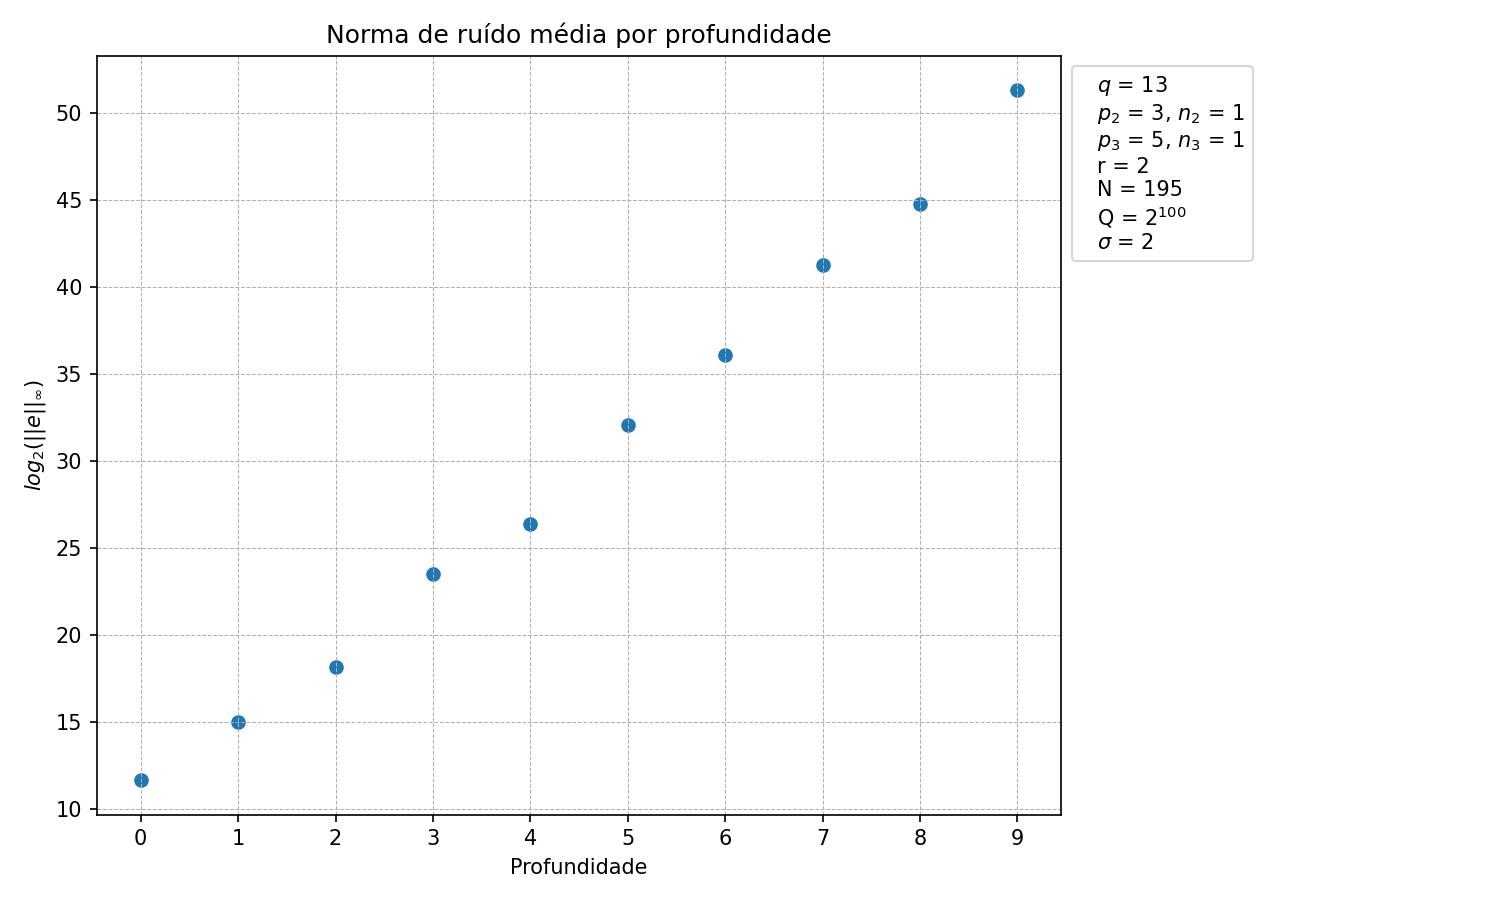
\includegraphics[width=0.8\textwidth]{images/wrong_packing.jpg}
    \caption{Crescimento do ruído pela quantidade de produtos externos com empacotamento errado.}
    \label{fig:wrong_packing}
\end{figure}

\newpage

\section{Traço homomórfico sobre RLWE}

O objetivo é encontrar uma maneira de executar o Eval-Trace, isto é, dado um criptograma $d \in \text{RLWE}_s(\mu)$ computar um criptograma 
$d' \in \text{RLWE}_s(Tr_{K/K_{13}}(\mu))$ homomorficamente, ou seja, sem ter acesso a mensagem original.

\subsection{Algoritmo de Key Switch}
Primeiramente, é necessário introduzir o conceito de troca de chave, \textit{key-switch}. Como está no nome, esse algoritmo tem por objetivo trocar a chave na qual um criptograma está crifrado. 

\subsubsection{Descrição matemática do Algoritmo}

\begin{enumerate}
    \item \textbf{Criptograma Original:} Um criptograma $\RLWE$ $c = (a, b) \in \mcR^2$ cifra uma mensagem $\mu$ sob a chave $s'$ se
    \[
        b = a \cdot s' + e + \mu \cdot \Delta
    \]
    onde $e$ é o ruído e $\Delta = Q/B$.

    \item \textbf{Chave de Troca de Chave ($K_{s' \to s}$):} É um conjunto de criptogramas $\{k_i\}$ que cifram múltiplos da antiga chave $s'$ sob a nova chave $s$.
    Cada $k_i \in K_{s' \to s}$ é um criptograma $\RLWE_s(s' \cdot g[i])$.

    \item \textbf{Procedimento:}
    \begin{itemize}
        \item Calcula-se um criptograma de $a \cdot s'$ sob a nova chave $s$ via
        \[
            (a_{\text{new}}, b_{\text{new}}) = \sum_{i=0}^{\ell-1} k_i \cdot g^{-1}(a)[i]
        \]
        \item Agora vamos calcular o criptograma procurado,
        \[
            c' = (-a_{\text{new}}, b - b_{\text{new}}).
        \]
    \end{itemize}

    \item \textbf{Verificação:} Decifrando $c' = (a', b')$ com a chave $s$, temos:
    \[
        b' + a' \cdot s = (b - b_{\text{new}}) - a_{\text{new}} \cdot s \approx b - (b_{\text{new}} + a_{\text{new}} \cdot s) \approx b - a \cdot s'.
    \]
    Como $b = a \cdot s' + e + \mu \cdot \Delta$, resulta que:
    \[
        b' + a' \cdot s \approx \mu \cdot \Delta + e.
    \]
    Ou seja, a mensagem $\mu$ (com ruído $e$) agora está cifrada sob a nova chave $s$.
\end{enumerate}

\subsubsection{Pseudocódigo e implementação do key switch}

\begin{algorithm}[H]
\caption{Algoritmo de Troca de Chave (Key-Switching)}
\label{alg:keyswitch}
\DontPrintSemicolon

\KwIn{
    Criptograma $c = (a, b) \in \mathcal{R}_Q^2$, uma cifra $\RLWE_{s'}(\mu)$.\;
    Chave de troca de chave $K_{s' \to s} = \{k_i = \RLWE_s(s' \cdot g_i)\}_{i=0}^{\ell-1}$.\;
}
\KwOut{
    Criptograma $c' \in \mathcal{R}_Q^2$, uma cifra $\RLWE_{s}(\mu)$.
}
$(a_0, a_1, \dots, a_{\ell-1}) \leftarrow g^{-1}(a)$ \\
$(a_{\text{new}}, b_{\text{new}}) \leftarrow (0, 0) \in \mathcal{R}_Q^2$.\\
\For{$i \leftarrow 0$ \KwTo $\ell-1$}{
    Seja $k_i = (c_i, d_i)$.\\
    $(a_{\text{new}}, b_{\text{new}}) \leftarrow (a_{\text{new}} + a_i \cdot c_i, b_{\text{new}} + a_i \cdot d_i)$.\\
}
$a' \leftarrow -a_{\text{new}}$.\\
$b' \leftarrow b - b_{\text{new}}$\\
\Return{$c' = (a', b')$}
\end{algorithm}

É claro que a implementação deste algoritmo é bem mais simples na prática. A seguir um snippet de código que contém não só a
implementação da troca de chave no RLWE como RGSW, com a única diferença é que temos que aplicar a diferença para as linhas 
relevantes.

\begin{minted}{python3}
def key_switch_rlwe(ciphertext, K, base, B, q, N):
    f = Zx(cyclotomic_polynomial(N))
    Zqx = ZZ.quotient(q)['x'] 
    Rq = Zqx.quotient(f)
    
    a, b = ciphertext[0], ciphertext[1]
    ev_aK = vector(inv_g_poly(a, base, q, N)) * K 
    
    ev_aK = [Rq(ev_aK[0]), Rq(-ev_aK[1])]
    return vector([-ev_aK[0], Rq(b) + Rq(ev_aK[1])])

def key_switch_gsw(gsw, K, base, C): 
    l, B, q, n = gsw.l, gsw.B, gsw.q, gsw.n
    new_C = Matrix(gsw.Rq, 2* l, 2)

    for i in range(l):
        new_C[l+i] = key_switch_rlwe(C[l+i], K, base, B, q, n)
        new_C[i] = gsw.inv_g_row_ciphertext(new_C[l+i]) * gsw.Ks

    return new_C
\end{minted}

\subsection{Pseudocódigo do algoritmo}

Basta apresentar o algoritmo utilizado para o Eval-trace, no pseudocódigo a seguir foi escolhido um traço em específico 
mas note que basta apenas trocá-lo pelo outro cenário.  


\begin{algorithm}[H]
\caption{(RLWE)-Eval-Tr\(_{K/K_{13}}\) com a estrutura de torre}
\SetKwInOut{Input}{Entrada}
\SetKwInOut{Output}{Saída}

\Input{
\begin{itemize}
  \item \(c = (b, a) \in (\mcR)^2\) que encripta uma mensagem \(\mu \in \mcR\) sob um segredo \(s \in \mathcal{R}\).
  \item \(\{\text{evk}^{(\sigma)}\}_{\sigma \in \bigcup_{i=1}^{t-1} \text{Gal}(E_i/E_{i+1})}\), e \(\text{evk} \in \text{RGSW}_s(P^{-1} \cdot s) \in \mathcal{R}^2\).
\end{itemize}
}
\Output{
\(c_{out} \in \text{RLWE}_s(\text{Tr}_{K/K_{13}}(\mu))\).
}

Inicialize \(c = (b, a)\)\\
Calcule \(d = \text{evk} \boxtimes (0, a)\) \\
\For{\(i = 1\) até \(t - 1\)}{
  Tome $(d_1, d_2) \gets d$\\
  Calcule \(d' = \sum_{\sigma \in \text{Gal}(E_i/E_{i+1})} \text{KS}( \sigma(d_1), \sigma(d_2), \text{evk}^{(\sigma^{-1})})\)\\
  Atualize $d = d'$ e $d' = (0,0)$
}
Retorne \((\text{Tr}_{K/K_{13}}(b), 0) - d\) 
\end{algorithm}

Perceba que como armazenamos os criptogramas já em $\mcR$ a multiplicação por tal fator aqui se torna desnecessária. Para computar
as chaves necessárias evk e as relativas ao key-switch, a classe que implementa o esquema RGSW calcula tais valores assim 
que instanciada.

Para mostrar sua corretude, observe que antes do loop $d \in \RLWE_s{as}$, durante o loop calculamos o traço encriptado $as$
com ajudar do key-switch. Logo, o algortimo retorna
$$
  (\text{Tr}_{K/K_{13}}(b - as) - a's - e, - a') = (-a's + \text{Tr}_{K/K_{13}}(\mu) \frac{Q}{B} + e' , -a')
$$
ou seja, um criptograma válido de $\RLWE_s(\text{Tr}_{K/K_{13}}(\mu))$.

\newpage

\subsection{Análise de Ruído das operações}

Nesta seção estão as análises do crescimento de ruído das operações entre criptogramas RLWE e RGSW.
\subsubsection*{Soma Homomórfica $C_1 \boxplus  C_2$}
O ruído dessa operação pode ser calculado por:
$$
Err(C_1 \boxplus  C_2) = sk^T(C_1 + C_2) - (\mu_1 + \mu_2)sk^TG
$$
Organizando,
$$
Err(C_1 \boxplus  C_2) = sk^T(C_1) - (\mu_1)sk^TG + sk^T(C_2) - (\mu_2)sk^TG = e_1^T + e_2^T 
$$

\subsubsection{Multiplicação Homomórfica $C_1 \boxdot C_2$}
O ruído desta operação pode ser calculado por
$$
Err(C_1 \boxdot C_2) = sk^\top(C_1G ^{-1}(C_2)) - (\mu_1\mu_2)sk^\top \mathbf{G}
$$
Expandindo a expressão encontra-se:
$$
Err(C_1 \boxdot C_2) = (1,-s) \begin{pmatrix} s \mathbf{a}_1^\top + \mathbf{e}_1^\top \\ \mathbf{a}_ 1^\top \end{pmatrix}G ^{-1}(C_2) + \mu_1(1,-s)\begin{pmatrix} s \mathbf{a}_2^\top + \mathbf{e}_2^\top \\ \mathbf{a}_ 2^\top \end{pmatrix}
$$
Simplificando, finalmente:
$$
Err(C_1 \boxdot C_2) = \mathbf{e}_1^\top G ^{-1}(C_2) + \mu_1 \mathbf{e}_2^\top
$$

O produto externo padrão entre RGSW e RLWE pode ser calculado por

$$C_1 \boxtimes c_2 = \begin{pmatrix} s \mathbf{a}_1^\top + \mathbf{e}_1^\top \\ \mathbf{a}_ 1^\top \end{pmatrix}g^{-1}(c_2) + \mu_1\mathbf{G}g^{-1}(c_2)$$ 
$$=\begin{pmatrix} s \mathbf{a}_1^\top g^{-1}(c_2) + \mathbf{e}_1^\top g^{-1}(c_2) \\ \mathbf{a}_ 1^\top g^{-1}(c_2) \end{pmatrix} + \begin{pmatrix} s a_2 \mu_1 + \mu_1 \mu_2 \frac{Q}{B} + \mu_1 e_2 \\ a_2 \mu_1 \end{pmatrix} $$
$$=\begin{pmatrix} s ( \mathbf{a}_1^\top g^{-1}(c_2) + a_2\mu_1) + \mu_1\mu_2\frac{Q}{B} +  \mathbf{e}_1^\top g^{-1}(c_2) +\mu_1 e_2 \\ \mathbf{a}_ 1^\top g^{-1}(c_2) + a_2 \mu_1 \end{pmatrix}$$
Finalmente, o ruído é calculado por:
$$
Err(C_1 \boxtimes c_2) = \mathbf{e}_1^\top g^{-1}(c_2) +\mu_1 e_2  
$$
Dessa forma, a sua norma infinita deve ser
$$
||Err(C_1 \boxtimes c_2)||_\infty < 2\ell N||e_1||_\infty + \mu_1 ||e_2||_\infty 
$$

\subsubsection{Subgaussiana}
Para a análise de ruído 'justa' é preciso utilizar que parte das variáveis aleatórias trabalhadas são limitadas por distribuições 
subgaussianas. A intuição é de que podemos encontrar um limite superior probabilístico utilizando a desigualdade de Markov se soubermos
a distribuição que rege a variável aleatória. 

\begin{definition}
    Para \( s > 0 \), define-se a função Gaussiana \( \rho_s : H \to (0,1] \) por
\[
\rho_s(\mathbf{x}) = \exp\left(-\pi \|\mathbf{x}\|_2^2 / s^2\right).
\]
A distribuição Gaussiana contínua \( D_s \) é obtida pela normalização de \( \rho_s \), com densidade \( s^{-n} \cdot \rho_s(\mathbf{x}) \).

Define-se também que uma variável aleatória \( X \in \mathbb{R} \) é \( \delta \)-subgaussiana com parâmetro \( s > 0 \) se, para todo \( t \in \mathbb{R} \),
\[
\mathbb{E}[\exp(2\pi t X)] \leq \exp(\delta + \pi s^2 t^2).
\]

\end{definition}

Agora tome as seguintes propriedades presentes em \cite{lyubashevsky2013} e \cite{lw23I}.

\begin{lemma}[Lema 3.2 \cite{lw23I}]
    \textit{Para quaisquer cifras RGSW} $\mathbf{C}_1, \mathbf{C}_2$ \textit{que cifram} $\mu_1, \mu_2$ \textit{com termos de erro} $\mathbf{e}_1, \mathbf{e}_2$ \textit{respectivamente, temos o seguinte:}

    \[
    \text{Err}(\mathbf{C}_1 \boxplus \mathbf{C}_2) = \mathbf{e}_1^\top + \mathbf{e}_2^\top.
    \]

    \[
    \text{Err}(\mathbf{C}_1 \boxtimes \mathbf{C}_2) = \mathbf{e}_1^\top \cdot \mathbf{G}^{-1}(\mathbf{C}_2) + \mu_1 \cdot \mathbf{e}_2^\top.
    \]

    \textit{Além disso, suponha que} $\mathbf{G}^{-1}$ \textit{é amostrado com respeito a alguma base} $\mathbb{Z}$ \textit{de} $\mathcal{R}$, \textit{isto é,} $\mathbf{B} = \{ \mathbf{b}_1, \dots, \mathbf{b}_n \}$, \textit{tal que} $\max_{i \in [n]} \{ \| \sigma(\mathbf{b}_i) \|_\infty \} \leq 1$ \textit{como no Lema 2.3. Então os seguintes fatos valem:}

    \begin{itemize}
    \item Denote $\mathbf{e}_1^\top \cdot \mathbf{G}^{-1}(\mathbf{C}_2)$ como $\mathbf{e}^\top = (e_1, \dots, e_{2\ell})$. Então cada entrada de $\mathbf{e}$ é uma variável aleatória independente.

    \item $\|\sigma(\mathbf{e})\|_\infty$ é limitada superiormente por uma variável sub-Gaussiana com parâmetro $O(r)$, para algum $r > 0$ tal que $r \leq \sqrt{N \cdot \log Q} \cdot \|\sigma(\mathbf{e}_1)\|_\infty$.
    \end{itemize}
\end{lemma}

\begin{lemma}
    Seja uma variável aleatória $X$ de distribuição gaussiana de parâmetros $(\mu = 0, \sigma)$, esta variável é limitada superiormente
    por um subgaussiana de parâmetro mínimo $\sqrt{2\pi}\sigma$
\end{lemma}

Com o último lema, garantimos que a amostragem gaussiana do erro reflete em uma variável subgaussiana. Logo, passamos para uma análise dos ruídos acumulados pelo resto das operações.

\subsubsection{Key Switch}
O algoritmo de key-switch, tem como função a troca de chave de um criptograma cifrado
em uma chave antiga $s'$, para uma chave nova $s$, o que aumenta o ruído gerado na cifra, vamos verificar quanto.
Para que o algortimo seja realizado corretamente, é necessário 
que seja passado como parâmetro a \textit{lower half} de um criptograma $RGSW_s(s')$, ou seja, é necessário assumir 
que o RGSW tem segurança circular.

Seja então $d \in \text{RLWE}_{s'}(\mu)$ e $d = (a, b)$, e queremos então um criptograma de $\mu$ cifrado em $\text{RLWE}_{s}$.
Considere então $K$ a \textit{lower half} de um criptograma $RGSW_s(s')$. O objetivo então é encontrar o ruído gerado por, 
$$
[0,b] - K \times g^{-1}(a)
$$
Como $K$ é a parte inferior de $RGSW_s(s')$ considere $K = (A, As + gs' + \mathbf{e}_{KS}) \in \mathcal{R}_Q^{2 \times \ell}$. Desenvolvendo,

$$
-(g^{-1}(a) \times A), -(g^{-1}(a) \times A) s + \mu \frac{Q}{B} + E - \mathbf{e}_{KS} g^{-1}(a)
$$
Note que o vetor obtido é um criptograma valido $\in \text{RLWE}_{s}(\mu)$ com ruído 
$E - \mathbf{e}_{KS} g^{-1}(a)$ que possui norma infinita correspondente:
$$
||Err(KS(d))||_\infty < ||Err(d)||_\infty + N\ell ||\mathbf{e}_{KS}||_\infty
$$
No teorema 4.6 de \cite{lw23I}, assume-se que $Err(d)$ e $\mathbf{e}_{KS} g^{-1}(a)$ são subgaussianas com um mesmo parametro $B$, o que é coerente visto que a magnitude do ruído do key-switch deve ser muito menor do que a da mensagem $d$. O key switch foi implementado em SageMath e C++.

\subsubsection{Eval-Trace}

Para facilitar a análise de ruído do algoritmo 4.1 de \cite{lw23I}, considere o mesmo
algoritmo simplificado, para o efeito da acumulação do ruído ser mais visível, a variável $d$ terá um 
índice que representa seu degrau na torre de extensão. 

\begin{algorithm}[H]
\caption{(RLWE)-Eval-Tr\(_{K/K_{13}}\) com a estrutura de torre}
\SetKwInOut{Input}{Entrada}
\SetKwInOut{Output}{Saída}

\Input{
\begin{itemize}
  \item \(c = (b, a) \in (\mathcal{R}_1 \otimes \mathcal{R}_2 \otimes \mathcal{R}_3)^2\) que encripta uma mensagem \(\mu \in \mathcal{R}_1 \otimes \mathcal{R}_2 \otimes \mathcal{R}_3\) sob um segredo \(s \in \mathcal{R}\).
  \item \(\{\text{evk}^{(\sigma)}\}_{\sigma \in \bigcup_{i=1}^{t-1} \text{Gal}(E_i/E_{i+1})}\), e \(\text{evk} \in \text{RGSW}_s(P^{-1} \cdot s) \in \mathcal{R}^2\).
\end{itemize}
}
\Output{
\(c_{out} \in \text{RLWE}_s(\text{Tr}_{K/K_{13}}(\mu))\).
}

Inicialize \(c = (b, a)\), defina \(\bar{a} = P \cdot a\) \\
Calcule \(d_0 = \text{evk} \boxtimes (0, \bar{a})\) \\
\For{\(i = 1\) até \(t - 1\)}{
  Calcule \(d_{i+1} = \sum_{\sigma \in \text{Gal}(E_i/E_{i+1})} \text{KS}( \sigma(d_i), \text{evk}^{(\sigma^{-1})})\)\\
}
Retorne \((\text{Tr}_{K/K_{13}}(b), 0) - d_n\) 

\end{algorithm}
Assuma sem perda de generalidade que o traço realizado é $K \rightarrow K_{13}$.
Começaremos analisando a recurssão do loop na linha 4:
$$
d_{i+1} = \sum_{\sigma \in \text{Gal}(E_i/E_{i+1})} \text{KS}( \sigma(d_i), \text{evk}^{(\sigma^{-1})})
$$
Então, utilizando a expressão do erro do key-switch:
$$
Err(d_{i+1}) = \sum_{\sigma \in \text{Gal}(E_i/E_{i+1})} Err(\sigma(d_i)) - e_{KS}^{\sigma} g^{-1}(d_i[0])
$$
Perceba que $Err(\sigma(d_i)) = \sigma(Err(d_i))$ e que o segundo termo no somatório tem sua norma limitada por um valor pequeno,
em uma análise inicial $N\ell ||e_{KS}^{\sigma}||$, utilizando o lema 3.2 é uma variável subgaussiana com parâmetro limitado por 
$\sqrt{N\ell} ||e_{KS}^{\sigma}||$. Visto que sua norma independe do seu estágio na torre, troque-o por $e'$ onde $||e'|| \le  N\ell ||e_{KS}^{\sigma}||$. Logo, 
$$
Err(d_{i+1}) < p_2 e'+ \sum_{\sigma \in \text{Gal}(E_i/E_{i+1})} \sigma(Err(d_i))
$$
Observe que o termo $\sum_{\sigma \in \text{Gal}(E_i/E_{i+1})} \sigma(Err(d_i)) = Tr_{E_i / E_{i+1}}(Err(d_i))$ 
$$
Err(d_{i+1}) < p_2 e' + Tr_{E_i/E_{i+1}}(Err(d_i))
$$
A partir dessa recorrência, é possível chegar na relação:
$$
Err(d_{n}) < Tr_{K / K_{13}}(Err(d_0)) + \rho' e'
$$
Sabendo que $d_0 = evk \boxtimes [0, \bar{a}]$, $Err(d_0) = Err(evk) g^{-1}([0, \bar{a}])$.
Tome $f$ como o criptograma resultante, $f = (\text{Tr}_{K/K_{13}}(b), 0) - d_n$. Então, expressão  do ruído toma a forma:
$$
Err(f) < Tr_{K / K_{13}}(e) + Tr_{K /K_{13}}(Err(d_0)) + \rho' e'
$$
Ao considerar que as normas de ruído de $\mathbf{e}_{KS}$ e $evk$ são limitadas pelo mesmo valor $E$, temos que $||Tr_{K /K_{13}}(Err(d_0))|| < 2N \ell E$, logo
aplicando as normas:
$$
||Err(f)|| < ||Tr_{K /K_{13}}(e)|| +  3 \rho'N\ell E
$$

Lembrando que $||e||$ é a norma do ruído do criptograma inicial. Note que no teorema 4.6 de \cite{lw23I} é proposta uma análise mais justa do erro, a única 
diferença é que os produtos da forma $\mathbf{e} g^{-1}(x)$, onde $||\mathbf{e}|| < E$ são subgaussianos com parametros limitados. Tal operação foi implementada em SageMath e C++.

\subsubsection{\emph{framework} Ext-Prod}
Tome $\delta_i^{(j)}$ como a componente $i$ do ruído da mensagem $\mu_i^{(j)}$ empacotada cifrada em RGSW e  $e_i^{(j)}$ como a componente $i$ do ruído da mensagem $d_j$ resultante empacotada em RLWE. 

Analisado o resultado após Com o resultado da seção anterior e com o erro do produto externo, temos:
$$
e^{(1)} < Tr_{K / K_{13}}(\sum_i \delta_i^{(1)} v_i^v w_i g^{-1}(d_0) + \mu^{(0)} e_i^{(0)}v_i) +  \Delta
$$
Onde $||\Delta|| < 3 \rho'N\ell E$. Se aplicarmos a norma infinita da expressão, conseguimos obter:
$$
||e^{(1)}|| < \frac{2\rho (p_2-1)N\ell}{\rho'}\sum ||\delta_i^{(1)}|| + \rho ||\mu^{(1)}||\sum||e_i^{(0)}|| + 3 \rho'N\ell
$$
Perceba que essa expressão é análoga a expressão obtida no artigo ao efetuarmos uma análise utilizando variáveis subgaussianas.

\subsubsection{$k$ Aplicações}
Calcular o ruído após $k$, com $k$ par, operações onde as mensagens são $\mu_i^{(j)} = \xi_q^{t^{(j)}_i}$ simulando o que ocorre durante o batch bootstraping. Substituindo a expressão [], pelas variáveis definidas:
$$
e^{(k)} < \sum_i e_i^{(k-1)} \xi_q^{t^{(k)}_i} w_i + Tr_{K / K_{13}}(\sum_i \delta_i^{(k)} v_i^v w_i g^{-1}(d_{k-1})) +  \Delta
$$
Vamos replicar a mesma coisa para $k-1$ lembrando que agora o traço efetuado será relativo ao corpo $K_{12}$:
$$
e^{(k-1)} < \sum_i e_i^{(k-2)} \xi_q^{t^{(k-1)}_i} v_i + Tr_{K / K_{12}}(\sum_i \delta_i^{(k)} w_i^v v_i g^{-1}(d_{k-2})) + \Delta'
$$
onde $||\Delta'|| \le 3 \tau'N\ell E$. Agora temos que isolar as componentes de $e^{(k-1)}$ utilizando o traço, por definição do dual temos:
$$
e_i^{(k-1)} = Tr_{K /K_{13}} (e^{(k-1)} v_i^v)
$$
Desenvolvendo este sistema, encontramos o resultado que:
$$
||e^{(k)}|| < ||e^{(0)}||+ \frac{k}{2}(4 p_2p_3r^2 + 6 p_2r \tau' + 2r p_2 + 3 \rho' ) N (\log Q) E
$$
Sobre a análise 'justa', utilizando o lema 8.3, basicamente o que mudam são as normas das operações envolvendo os vetores $g$, artigo ajustasse o parâmetro da subgaussiana para $r \sqrt{N \log Q} E$ tendo assim como resultado final:  
$$
||e^{(k)}|| < ||e^{(0)}||+ \frac{k}{2}(4 p_2p_3r^2 + 6 p_2r \tau' + 2r p_2 + 3 \rho' ) r \sqrt{N \log Q} E
$$
Note que esta operação foi implementada em SageMath e C++. Observe as figuras a seguir comparando o crescimento da norma infinita do ruído:

\begin{figure}[H]
  \centering
  \begin{subfigure}{0.45\textwidth}
    \centering
    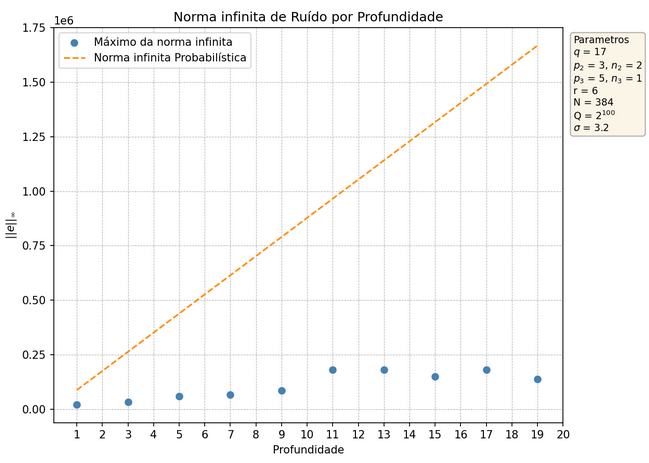
\includegraphics[width=\linewidth]{sections/images/image2.png}
  \end{subfigure}
  \hfill
  \begin{subfigure}{0.45\textwidth}
    \centering
    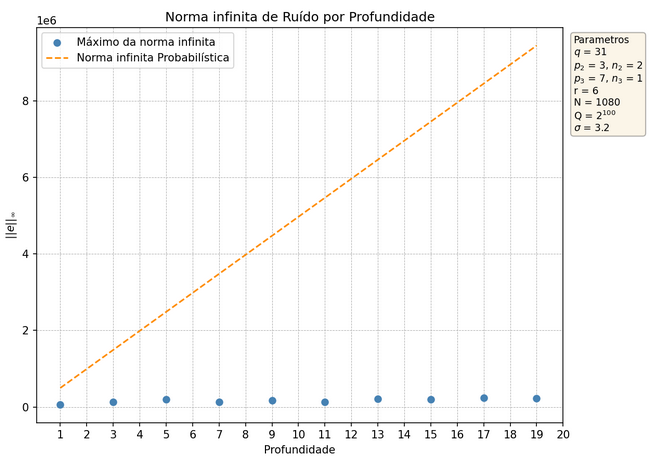
\includegraphics[width=\linewidth]{sections/images/image.png}
  \end{subfigure}
  \caption{Gráficos da norma infinita pela quantidade de produtos externos realizados }
\end{figure}

Para a geração destes \emph{plots} foram omitidas as constantes dos primos, levou-se em conta apenas as variáveis relacionadas ao parâmetro de segurança, $O(r^3\sqrt{N\log Q}E)$. Perceba que mesmo assim, existe uma distância bem razoável entre o ruído encontrado e o limite probabilistíco encontrado. Dado estes e outros testes, é um bom indicativo que escolher os parâmetros da forma utilizada pelo artigo, com a constante da análise assintótica sendo $1$ é, de fato, condizente com a realidade.



\newpage

\section{Complexidades e Definições de parâmetro}

\subsection{Complexidade de Memória}
Trivialmente, um inteiro com tamanho máximo $Q$ pode ser representado por $\log Q$ bits. Logo um polinômio de grau $N$ com seus coeficientes de tamanho 
máximo a $N \log Q$

\begin{itemize}
    \item RGSW: $2N \log^2 Q (\text{evk}) + [\phi(m_2) + \phi(m_3)] \log Q (\text{Automorfismos}) + [\phi(m_2) + \phi(m_3)] 2 N \log^2 Q (\text{KS}) + 
    6 \log Q (\text{máximo superestimado}) \approx O(r N \log^2 Q)$
    \item RLWE $6 \log Q (\text{máximo superestimado})$
    \item chaves $4 N \log Q (\text{máximo superestimado})$
    \item Total parece ser proporcional a $\approx O(r N \log^2 Q)$
\end{itemize}

Criptogramas RGSW $4 N \log^2 Q$ / Criptogramas RLWE $2N \log Q$

\subsection{Complexidade de Tempo}

Produto externo + Traço

    
Produto Externo:
\begin{itemize}
    \item Decompor dois polinomios, decompor $\phi(N)$ vezes a complexidade de decompor um inteiro na base necessária (base normalmente é 2) 
    \item Multiplicar um vetor de $(1 \times 2\ell)$ por uma matrix $(2\ell \times 2)$ onde cada indíce é um polinômio representado por $N \log Q$ bits,
    basicamente $4 \ell$ multiplicações e $4\ell - 2$ adições.
\end{itemize}

Traço Homomórfico:
\begin{itemize}
    \item Produto externo
    \item Se o corpo reduzido tem como potência de primo $m$, vamos ter $\log d$ chamadas de key-switch, cada key switch faz $2\ell$ multiplicacoes e $2\ell - 2$ somas.
    
    No total seria algo como $\log d \times (2 \ell \text{ multiplicações} + 2 \ell \text{ adições}) $
\end{itemize}

\newpage

\begin{thebibliography}{9}
    \bibitem{lyubashevsky2013}
    Lyubashevsky, V., Peikert, C., Regev, O.:
    \textit{A toolkit for ring-LWE cryptography}.
    In: Johansson, T., Nguyen, P.Q. (eds.) EUROCRYPT 2013. LNCS, vol. 7881, pp. 35–54. Springer, Heidelberg (2013).
    Available at: \url{https://eprint.iacr.org/2013/293.pdf}
    
    \bibitem{lw23I}
    Liu, F.-H., Wang, H.:
    \textit{Batch Bootstrapping I: A New Framework for SIMD Bootstrapping in Polynomial Modulus.} 
    In: Advances in Cryptology -- EUROCRYPT 2023: 42nd Annual International Conference on the Theory and Applications of Cryptographic Techniques, 
    Lyon, France, April 23–27, 2023, Proceedings, Part III, pp. 321–352. 
    Springer, Berlin, Heidelberg (2023). 
    Available at: \url{https://doi.org/10.1007/978-3-031-30620-4_11}
    
    \bibitem{lw23II}
    Liu, F.-H., Wang, H.:
    \textit{Batch Bootstrapping II: Bootstrapping in Polynomial Modulus only Requires Õ(1) FHE Multiplications in Amortization.}
    In: Advances in Cryptology -- EUROCRYPT 2023: 42nd Annual International Conference on the Theory and Applications of Cryptographic Techniques, 
    Lyon, France, April 23–27, 2023, Proceedings, Part III, pp. 353–384. 
    Springer, Berlin, Heidelberg (2023). 
    Available at: \url{https://doi.org/10.1007/978-3-031-30620-4_12}
    
    \bibitem{BrakerskiEtAl2013}
    Brakerski, Z., Langlois, A., Peikert, C., Regev, O., Stehlé, D.: Classical hardness of learning with errors. In: Boneh, D., Roughgarden, T., Feigenbaum, J. (eds.) 45th ACM STOC, pp. 575--584. ACM Press (2013)

    \bibitem{Balbas2021}
    Balbás, D.: The Hardness of LWE and Ring-LWE: A Survey. Cryptology ePrint Archive, Paper 2021/1358 (2021)

    \end{thebibliography}
\end{document}